% Unicode source. Compile with Tectonic or XeLaTeX after python -m vlm_probe.depth report.
\documentclass[11pt,a4paper]{article}
\usepackage[margin=18mm,top=16mm,bottom=16mm]{geometry}
\usepackage{fontspec}
\IfFontExistsTF{Times New Roman}{\setmainfont{Times New Roman}}{\setmainfont{TeX Gyre Termes}}
\usepackage{amsmath,booktabs,caption,titlesec,graphicx}
\usepackage[unicode,hidelinks]{hyperref}
\hypersetup{pdftitle={Thăm dò chuyên sâu CLIP: quan hệ không gian và thông tin category},pdfauthor={Dự án ComputerVision Probing VLM}}
\renewcommand{\tablename}{Bảng}
\renewcommand{\figurename}{Hình}
\renewcommand{\refname}{Tài liệu tham khảo}
\titleformat{\section}{\normalsize\bfseries}{\thesection.}{0.5em}{}
\titleformat{\subsection}{\normalsize\bfseries}{\thesubsection.}{0.5em}{}
\titlespacing*{\section}{0pt}{7pt}{3pt}
\titlespacing*{\subsection}{0pt}{5pt}{2pt}
\captionsetup{font=small,labelfont=bf,skip=4pt}
\setlength{\parindent}{0pt}\setlength{\parskip}{4pt}
\setlength{\tabcolsep}{7pt}\renewcommand{\arraystretch}{1.12}
\hyphenpenalty=10000\emergencystretch=2em
\newcommand{\SyntheticAcc}{27,36}
\newcommand{\NaturalAcc}{28,00}
\newcommand{\NaturalCI}{[22,00; 34,50]}
\newcommand{\NaturalFlipBoth}{10,50}
\newcommand{\NaturalHorizontalBoth}{3,00}
\newcommand{\NaturalOrderAgreement}{15,00}
\newcommand{\NaturalPairAssignment}{54,00}
\newcommand{\NaturalPairCI}{[45,00; 64,00]}

\begin{document}
\begin{center}
{\large\bfseries BÁO CÁO TIẾN ĐỘ — ĐỀ TÀI 14}\\[3pt]
{\Large\bfseries Thăm dò chuyên sâu CLIP: quan hệ không gian\\ và tác động của thông tin nhóm lớp}\\[4pt]
{\small Computer Vision \quad|\quad Cập nhật: 04/11/2026}
\end{center}
\vspace{-4pt}
\textbf{Tóm tắt.} Nghiên cứu tiếp nối đánh giá một checkpoint CLIP ViT-B/32 bằng các can thiệp giữ nguyên vật thể nhưng đổi quan hệ, cách viết và thuộc tính phụ; đối chứng thông tin nhóm lớp trên CIFAR-100; kiểm chứng trên ảnh tự nhiên. Mô hình nhận dạng màu/hình tốt nhưng thiếu nhất quán về quan hệ. Category đúng tốt hơn category sai, song giảm accuracy so với baseline. Hiện tượng thiếu nhất quán lặp lại trên tập COCO nhỏ đã lọc, trong khi hướng thiên lệch đáp án thay đổi. Kết quả mô tả hành vi của checkpoint được kiểm tra, chưa xác định cơ chế bên trong mô hình.

\section{Câu hỏi nghiên cứu và phương pháp}
Giữ cố định OpenAI CLIP ViT-B/32~\cite{clip}, trọng số, preprocessing, FP32/QuickGELU và batch 32; không fine-tuning. Dự đoán bằng cosine giữa vector ảnh và các vector mô tả đã chuẩn hóa. Năm baseline trước đây gồm CIFAR-100 (64,48\%), Flowers102 (63,77\%), Oxford-IIIT Pet (85,06\%), DTD partition 1 (42,45\%) và Food-101 (82,31\%), tổng 46.948 ảnh test.

Ba câu hỏi: \textbf{RQ1}, dự đoán quan hệ có đổi đúng và nhất quán khi can thiệp vào ảnh/câu? \textbf{RQ2}, thông tin category thay đổi cạnh tranh giữa các lớp như thế nào? \textbf{RQ3}, hiện tượng có lặp lại trên ảnh tự nhiên? Giả thuyết hình thành sau khi xem kết quả core; giao thức bổ sung được ghi trước suy luận tương ứng. Tập CIFAR-100 đã được quan sát trước nên không xem đây là tập xác nhận mới.

Hình học gồm 120 nhóm cảnh, mỗi nhóm có ba biến thể màu/hình và bốn quan hệ trái/phải/trên/dưới: \textbf{1.440 ảnh, 8.640 phép thử}. Ba mẫu câu: T0 ``a drawing of A r B'', T1 ``A is r B'', T2 ``an image of A r B''; mỗi câu có bản đảo A/B và đảo quan hệ để giữ nghĩa. Điểm đúng trừ đối thủ mạnh nhất là margin. Mọi đáp án được quy về cùng quan hệ A--B trước khi so sánh. CI 95\% dùng bootstrap 2.000 lần, seed 1402, lấy mẫu theo nhóm cảnh; category dùng bootstrap ghép cặp phân tầng lớp; ảnh tự nhiên dùng ảnh nguồn làm nhóm. CI không hiệu chỉnh đa so sánh.

\section{RQ1: Can thiệp quan hệ và tính nhất quán}
\begin{center}
\captionof{table}{Accuracy (\%) và CI 95\% theo cách viết. Hình học dùng 1.440 ảnh; tự nhiên chỉ 200 ảnh gốc. Mốc ngẫu nhiên: 25\%. T0 tự nhiên dùng ``photo'' thay ``drawing''.}
\label{tab:spatial}
\small
\begin{tabular}{@{}lrrrr@{}}
\toprule
Mẫu câu/thứ tự & Hình học & CI 95\% & Tự nhiên & CI 95\% \\
\midrule
T0 / thuận & 27,36 & [26,18; 28,61] & 26,00 & [20,00; 32,00] \\
T0 / đảo tương đương & 26,25 & [25,42; 27,15] & 27,00 & [21,00; 33,00] \\
T1 / thuận & 24,93 & [24,38; 25,49] & 24,50 & [18,50; 30,50] \\
T1 / đảo tương đương & 25,49 & [24,93; 26,04] & 22,00 & [17,00; 27,51] \\
T2 / thuận & 24,72 & [23,75; 25,69] & 28,00 & [22,00; 34,50] \\
T2 / đảo tương đương & 23,68 & [22,64; 24,65] & 24,50 & [18,50; 30,50] \\
\bottomrule
\end{tabular}

\end{center}
\vspace{-5pt}
Điều kiện chính T0 thuận đạt \textbf{\SyntheticAcc\%}, trong khi đối chứng nhận dạng màu/hình đạt \textbf{96,94\%}. Ngay trên phần nhận dạng đúng, quan hệ chỉ đạt 27,51\%. Cặp trái/phải cùng đúng là \textbf{2/360 (0,56\%)}, cặp trên/dưới cùng đúng là \textbf{6/360 (1,67\%)}; không nhóm nào đúng cả bốn vị trí. Hai cách viết tương đương T0 cho cùng dự đoán ở 16,25\% ảnh, cùng đúng ở 2,99\%. Khi chỉ đổi màu/hình, 17,92\% bộ ba giữ cùng dự đoán và 4,79\% đúng cả ba.

Mô hình chọn ``trên'' ở 809/1.440 ảnh (56,18\%), dù nhãn cân bằng. Tuy nhiên, dự đoán chỉ trùng nền trống ở 23,82\% ảnh; dữ liệu không hỗ trợ giải thích toàn bộ lỗi bằng một đáp án ưu tiên khi không có vật thể. Các kết quả cho thấy khoảng cách giữa nhận dạng và kết hợp quan hệ, đồng thời phản ứng với thông tin không quyết định nhãn. Chưa thể quy lỗi cho riêng bộ mã hóa ảnh hay văn bản.

\newpage
\section{RQ2: Đối chứng thông tin nhóm lớp trên CIFAR-100}
Luôn phân loại đủ 100 lớp trên cùng 10.000 ảnh. So sánh baseline ``a photo of a \{class\}'' với phần thêm ``a type of \{category\}'', suffix trung tính, và năm ánh xạ category sai cố định (seeds 271--275). Ánh xạ sai giữ phân bố cụm category, không để lớp nào giữ lại category đúng. Suffix trung tính chọn chỉ theo tokenizer: 80 lớp khớp số token, 20 lớp lệch một token. Đây là kiểm soát độ dài một phần, không tách hoàn toàn cú pháp/ngữ nghĩa.

\begin{center}
\captionof{table}{Kết quả tám điều kiện. Chênh lệch tính bằng điểm phần trăm so với baseline. Top-1 bằng macro do mỗi lớp có 100 ảnh.}
\label{tab:category}
\begin{tabular}{@{}lrr@{}}
\toprule
Điều kiện & Accuracy (\%) & Chênh lệch \\
\midrule
Baseline & 64,48 & 0,00 \\
Category đúng & 62,92 & -1,56 \\
Nội dung trung tính & 64,09 & -0,39 \\
Category sai, seed 271 & 52,21 & -12,27 \\
Category sai, seed 272 & 54,31 & -10,17 \\
Category sai, seed 273 & 55,76 & -8,72 \\
Category sai, seed 274 & 53,25 & -11,23 \\
Category sai, seed 275 & 55,40 & -9,08 \\
\bottomrule
\end{tabular}

\end{center}
\vspace{-4pt}
Category đúng kém baseline \textbf{1,56 điểm \%}, CI [−2,14; −0,98], và kém trung tính \textbf{1,17 điểm \%}, CI [−1,77; −0,61]; nhưng tốt hơn trung bình năm ánh xạ sai \textbf{8,734 điểm \%}, CI [8,140; 9,330]. Trung tính−baseline có CI [−0,92; 0,11], chưa đủ kết luận hai phương pháp tương đương. Các CI trên lấy biến thiên theo ảnh, có điều kiện trên năm ánh xạ đã chọn.

Điểm lớp đúng trung bình tăng 0,001628 nhưng điểm đối thủ mạnh nhất tăng 0,002908, làm margin giảm 0,001280. Đối thủ mạnh nhất đổi lớp ở 33,75\% ảnh; nếu giữ đối thủ baseline cố định, thay đổi điểm trung bình là −0,000111. Vì vậy, không diễn giải rằng cùng một đối thủ luôn được nâng điểm. Có 416 ảnh sai thành đúng nhưng 572 ảnh đúng thành sai; 45 lớp tăng, 50 giảm, 5 không đổi. Lỗi trong nhóm tăng 1.335→1.387 và lỗi khác nhóm tăng 2.217→2.321: suy giảm không chỉ đến từ phân biệt các lớp cùng nhóm.

\textbf{Kết luận RQ2.} Tính phù hợp của category có ảnh hưởng, nhưng category đúng theo cấu trúc câu này không cải thiện baseline. Quan sát điểm lớp đúng riêng lẻ có thể gây hiểu sai vì quyết định phụ thuộc cạnh tranh với mọi lớp khác. Baseline/category chạy lại khớp toàn bộ nhãn và scores cũ trên máy hiện tại.

\section{RQ3: Kiểm chứng trên ảnh tự nhiên}
Nguồn COCO val2014~\cite{coco}; lọc theo box tách biệt, quan hệ rõ, hai vật thể khác loại, không crowd và nằm trọn center crop. Nguồn đổi từ val2017 sang val2014 trước suy luận do val2017 chỉ có 70 ảnh đạt bộ lọc; giữ nguyên ngưỡng hình học. Rà soát 400 ứng viên, nhận 258, lấy 50 ảnh đầu mỗi quan hệ theo thứ tự hash đã cố định: \textbf{200 ảnh gốc}. Thêm bản lật ngang thành 400 ảnh đầu vào và 2.400 phép thử. Không chọn ảnh theo điểm CLIP.

T2 thuận là điều kiện chính chốt trước: \textbf{\NaturalAcc\%}, CI \NaturalCI\%, bao gồm mốc ngẫu nhiên 25\%. Chọn ``phải'' ở 124/200 ảnh (62\%), khác hướng ``trên'' của hình học. Hai cách viết tương đương T2 cùng dự đoán ở \NaturalOrderAgreement\% trong 400 ảnh đầu vào. Gốc/lật cùng đúng ở \NaturalFlipBoth\% của 200 cặp; riêng 100 cặp trái/phải bắt buộc đổi nhãn, chỉ \textbf{\NaturalHorizontalBoth\%} cùng đúng. Bản lật không được xem là nguồn ảnh độc lập; quan hệ trên/dưới giữ nguyên khi lật.

\textbf{Kết luận RQ3.} Sự thiếu nhất quán xuất hiện cả ngoài hình học, nhưng hướng thiên lệch không khái quát giữa hai miền. CI rộng không chứng minh mô hình tương đương đoán ngẫu nhiên. Chưa có đối chứng nhận dạng vật thể riêng trên COCO nên không quy mọi lỗi tự nhiên thuần túy cho quan hệ.

\newpage
\begin{center}
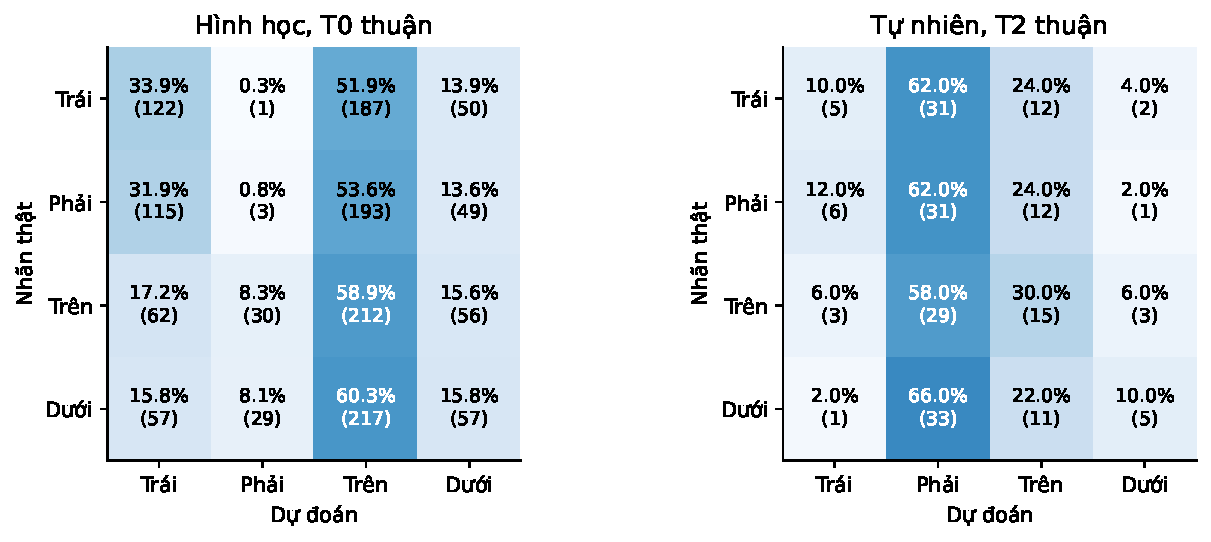
\includegraphics[width=0.85\linewidth]{spatial_confusion.pdf}
\captionof{figure}{Ma trận nhầm lẫn của hai điều kiện chính. Mỗi hàng là nhãn thật; số trong ngoặc là số ảnh. Hình học cân bằng 360 ảnh mỗi quan hệ, tự nhiên cân bằng 50 ảnh.}
\end{center}
\vspace{-3pt}
\section{Phân tích thăm dò bổ sung và các kết quả không ủng hộ giả thuyết}
Sau khi thấy accuracy thấp và lệch đáp án, bổ sung phép ghép hai ảnh đổi vị trí với hai caption tương ứng, tham khảo hướng đánh giá tính kết hợp ảnh--text~\cite{winoground}, không tái lập Winoground. Với ma trận cosine $S$, tính
\[
 D=S_{11}+S_{22}-S_{12}-S_{21}.
\]
$D>0$ nghĩa ghép đúng có tổng điểm cao hơn ghép chéo. Thành phần cộng chỉ phụ thuộc từng ảnh hoặc từng caption sẽ triệt tiêu; không loại mọi loại thiên lệch. Bài này có hai cách ghép, biết trước trục quan hệ, mốc ngẫu nhiên 50\%; không so trực tiếp với accuracy bốn lựa chọn.

T0 thuận hình học ghép đúng 45,00\% cặp ngang và 42,50\% cặp dọc. T2 thuận tự nhiên đạt \NaturalPairAssignment\% trên 100 cặp ngang, CI \NaturalPairCI\%. Chưa có bằng chứng mạnh về tín hiệu ghép đúng sau phép loại thành phần cộng này. Kết quả thu hẹp giải thích ``chỉ do một caption có điểm cao cố định'', nhưng không chứng minh encoder hoàn toàn không chứa thông tin vị trí. Đây là \textbf{phân tích hậu nghiệm}, công bố đủ các điều kiện, chưa phải xác nhận độc lập.

Phân tích core: đếm với bán kính cố định đạt 32,41\%, tổng diện tích cố định đạt 33,33\%; phủ định đạt 91,39\% với \emph{with/without} nhưng 80,83\% với \emph{contains/does not contain}. Chỉ 58,61\% nhóm đúng cả hai trạng thái và hai mẫu câu. Không thể kết luận tuyệt đối CLIP không xử lý được phủ định.

\section{Giới hạn, khả năng tái lập và công việc tiếp theo}
Nghiên cứu chỉ dùng một checkpoint và số hữu hạn cách viết/cảnh; CI phản ánh lấy mẫu trong tập hiện tại, không bao phủ mọi prompt, mapping hoặc miền ảnh. Category sử dụng lại test đã xem; không chọn prompt tối ưu rồi coi điểm trên cùng test là kiểm chứng độc lập. Tập tự nhiên được lọc chặt, nhãn là vị trí 2D; không khẳng định COCO chưa xuất hiện trong pretraining. Lật ảnh có thể thay đổi yếu tố khác ngoài quan hệ.

\textbf{Giới hạn nhãn tự nhiên:} rà soát trực quan do một trợ lý AI, kết hợp validator hình học từ annotation, không phải hai người gán nhãn độc lập; chưa đo đồng thuận. Mọi quyết định nhận/loại đã lưu trước suy luận. Ảnh giữ giấy phép riêng theo metadata; repository lưu URL/hash và kết quả, không phân phối lại ảnh.

Đã hoàn thành smoke/full và audit từ scores; 37 kiểm thử đạt. Baseline/category khớp 10.000/10.000 nhãn và scores cũ trên máy hiện tại. Lưu config, môi trường, checksum, nguồn mã và dự đoán từng mẫu. Bảng~\ref{tab:spatial}--\ref{tab:category} sinh từ JSON đã audit; \texttt{sources.json} ghi nguồn số liệu; mã mới ở \texttt{vlm\_probe/depth/}.

Bước tiếp theo: người trong nhóm rà soát độc lập nhãn tự nhiên; chốt trước giả thuyết ghép 2×2 rồi kiểm chứng trên tập mới. Nếu chọn prompt/category khác, tách tập phát triển và tập xác nhận. Prompt ensemble và nội dung tiếng Việt/văn hóa Việt Nam chưa thực hiện.

\begingroup\small
\begin{thebibliography}{3}
\setlength{\itemsep}{0pt}\setlength{\parskip}{0pt}
\bibitem{clip} A. Radford và cs., \href{https://proceedings.mlr.press/v139/radford21a.html}{``Learning Transferable Visual Models From Natural Language Supervision,''} \emph{ICML}, 2021.
\bibitem{coco} T.-Y. Lin và cs., \href{https://arxiv.org/abs/1405.0312}{``Microsoft COCO: Common Objects in Context,''} \emph{ECCV}, 2014.
\bibitem{winoground} T. Thrush và cs., \href{https://arxiv.org/abs/2204.03162}{``Winoground: Probing Vision and Language Models for Visio-Linguistic Compositionality,''} \emph{CVPR}, 2022.
\end{thebibliography}\endgroup
\end{document}
